\chapter{Scomposizione del VAB}
Per il calcolo delle equazioni dinamiche del sistema siamo andati a considerare ogni singolo corpo rigido componente il sistema, calcolandone le grandezze fisiche di posizione e velocità, seguendo un approccio cartesiano. 
Nello specifico abbiamo considerato il sistema composto da:
\begin{itemize}
	\item Asta
	\item Utente a bordo dello chassis
	\item Chassis (nel corso della trattazione sarà chiamata talvolta anche base)
	\item Ruota (che poi sarà considerata con un contributo, essendo il VAB composto da due ruote)
\end{itemize}

Ognuno di questi corpi rigidi separati è individuato da un punto, che ne rappresenta il centro di massa (o baricentro del corpo stesso): avremo quindi questo insieme di punti caratterizzanti il sistema (figura ~\ref{fig:VAB_baricentri})

\begin{itemize}
	\item \textbf{$P_a$}
	\item \textbf{$P_b$}
	\item \textbf{$P_c$}
	\item \textbf{$P_r$}
\end{itemize}

\begin{figure}[h]
	\centering   	
	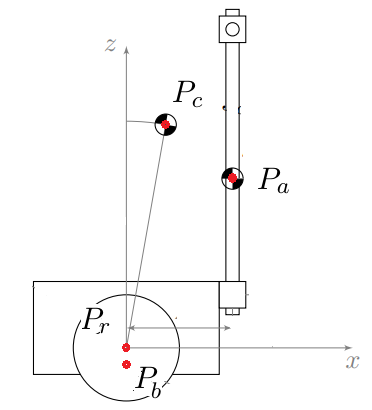
\includegraphics[width=0.4\textwidth]{Immagini/VAB_baricentrum.png}
	\caption{Baricentri dei singoli corpi rigidi}
	\label{fig:VAB_baricentri}
\end{figure} 

Prima di andare a definire le componenti di energia potenziale e cinetica di ogni singolo corpo, siamo andati ad introdurre alcune grandezze geometriche di supporto che definiremo qui di seguito.